\documentclass{article}
\usepackage{amsmath,amssymb,graphicx,tikz}
\usepackage{hyperref}
\usepackage{tikz}
\usepackage{amsfonts}
\usepackage{amsmath}
\usepackage{listings}

\title{CSC263 Winter 2016, Assignment 3}
\author{Connor Peet \#1001088208}
\renewcommand{\today}{~}
\hypersetup{pdfpagemode=Fullscreen,
  colorlinks=true,
  linkfileprefix={}}
\begin{document}
\maketitle

\lstset{
    numbers=left
}

\begin{enumerate}
\item [1.]
    Annotating the procedure steps:

    \begin{lstlisting}
Procedure nothing(A)
    A[1] := 0 # 1 step
    A[2] := 1 # 1 step
    for i = 3 to A.size do # multiply inside by (n - 2)
        s := 0 # 1 step
        for j = 1 to i - 1 do # multiply by (i - 1)
            s := s + A[j] # 1 step
        if A[i] is not equal to s then # 1 step
            return

    return
    \end{lstlisting}

    The worst input for the function is an array of integers, starting with $0$ and $1$, where each following integer is the sum of all previous integers, $[0, 1, 1, 2, 4, 8, ...]$. In this case, on an array with $n$ elements, the algorithm will not terminate until line 11 is reached and will take $2 + 2 \times (n - 2) \times \sum_{i = 1}^{n - 1} i$ steps.

    In the best case, the third element of the array is not $1$, causing the algorithm to terminate after the constant number of steps regardless of the total input size.
    \begin{enumerate}
    \item [(a)] The algorithm \textbf{is not} in $\mathcal{O}(n^2)$. Recall the formal definition of Big O. Taken from the CSC165 course notes, where $T_P(n)$ is the worst-case running time on an input of size $n$, it can be said
        \begin{gather*}
            T_P(n) \in \mathcal{O}(g) \text{ iff} \\
            \exists c \in \mathbb{R^+}, \exists B \in \mathbb{N}, \forall n \in \mathbb{N}, n \geq B \implies T_P(n) \leq cg(n)
        \end{gather*}
        \begin{itemize}
        \item We know the algorithm takes at most $2 + 2 \times (n - 2) \times \sum_{i = 1}^{n - 1} i$ steps. This is our worse-case running time.
        \item The summation can be evaluated from known definitions: $2 + 2 (n - 2) \times \frac{(n - 1) n}{2}$.
        \item The equation can be distributed: $2 + \frac{1}{2} (n - 2) \times (n^2 - n) = n^3 - 3n^2 + 2n + 2$.
        \item Then $T_P$ has in a cubic relationship to the input size.
        \item Then the algorithm is $\mathcal O(n^3)$, not $\mathcal O(n^2)$. A quick query on WolframAlpha lets us chose $c = 1$ and $B = 2$, which show this to be true.
        \end{itemize}
    \end{enumerate}
    \begin{enumerate}
    \item [(a)] The algorithm \textbf{is} $O(n^2)$. Recall the formal definition of Big Omega. Where $t_P(x)$ is the number of steps taken (running time) on input $x$,
        \begin{gather*}
            T_P(n) \in O(g) \text{ iff} \\
            \exists c \in \mathbb{R^+}, \exists B \in \mathbb{N}, \forall n \in \mathbb{N}, n \geq B \implies \\
            \exists x \in \text{Set of Program Inputs}, size(x) = n \land t_P(x) \geq cg(n)
        \end{gather*}
        \begin{itemize}
        \item In other words, we should be able to chose a $c$ and $B$ such that, for all input sizes $n$ greater than $B$, we can find an input that takes at least $cg(n)$ steps.
        \item In part (a) we showed that the worse input to the function takes $n^3 - 3n^2 + 2n + 2$ steps. This worst-case input $A_n$ can consistently be crafted for any given input size by the following procedure:
            \begin{itemize}
            \item If $n = 3$, then set $A_n = [0, 1, 1]$.
            \item If $n > 3$, then set $A_n = A_{n - 1} \cup \{ Sum(A_{n - 1}) \}$.
            \end{itemize}
        \item Therefore, picking $c = 1$ and $B = 2$, the algorithm satisfies the definition and is in $O(n^2)$.
        \end{itemize}
    \end{enumerate}

\item [2.]
    \begin{enumerate}
    \item [(a)]
        \begin{equation*}
        \begin{aligned}
            \textsc{Build-by-Inserts}([1, 2, 3, 2]) & \implies [3, 2, 2, 1] \\
            \textsc{Build-Max-Heap}([1, 2, 3, 2]) & \implies [3, 1, 2, 2]
        \end{aligned}
        \end{equation*}
    \item [(b)]
        \begin{itemize}
        \item The text states that \textsc{Max-Heap-Insert} runs in $\mathcal{O}(\log n)$ time.
        \item Then we can annotate the function as follows:
            \begin{lstlisting}
\textsc{Build-by-Inserts}(A)
    A.heap-size := 1 # 1 step
    for i := 2..n do # multiply inside by (n - 1)
        \textsc{Max-Heap-Insert}(A, A[i]) # at most log(n) steps
            \end{lstlisting}
        \item Then the function takes at most $1 + (n - 1) \log n$ steps, and is therefore in $\mathcal{O}(n \log n)$ time.
        \item But, we still need to show that it's in $O(n \log n)$ to assert that it's in $\Theta(n \log n)$.
        \item \textsc{Max-Heap-Insert} is in $O(\log n)$:
            \begin{itemize}
            \item The worst input of size $n$ to the function is an array of integers sorted from smallest to largest.
            \item In this case, the while loop in \textsc{Heap-Increase-Key} runs $\lfloor \log_2 n \rfloor$ times.
            \item Aside from the \textsc{Heap-Increase-Key} call, steps in \textsc{Max-Heap-Insert} are constant time.
            \item Also $\lfloor \log_2 n \rfloor < \log n$ for $n \geq 8$.
            \item Then \textsc{Max-Heap-Insert} is in $O(\log n)$
            \end{itemize}
        \item The \textsc{Max-Heap-Insert} function is called about $n$ times.
        \item Then the algorithm is in $O(n \log n)$.
        \item Then the algorithm is in $\Theta(n \log n)$.
        \end{itemize}
    \end{enumerate}
\item [3.]
    \begin{enumerate}
        \item [(a)] The set data $A$ is stored as an array bit triplets, where the index of the array (assuming indexing begins at zero) corresponds to the number represented by that index. From this, we will form a `sparse' but right-balanced binary search tree, with the node $\lfloor n / 2 \rfloor$ being the root. (Side note: the set sizes specified by the problem note that $n$ will always be a power of 2, but this data structure works for sets of any size.) \\

        For an empty tree, each item is a sequence of three bits set to zero, \texttt{000}. The middle bit determines whether or not the number represented by the current item is in the set. In the given tree that stores ${1, 2, 6}$, for instance, $A[1]$ would be \texttt{010} but $A[3]$ would be \texttt{000}. The left and right bits record whether, in the node's corresponding subtree, there exists \textit{any} active item. To illustrate:

            \begin{figure}[h]
                \begin{center}
                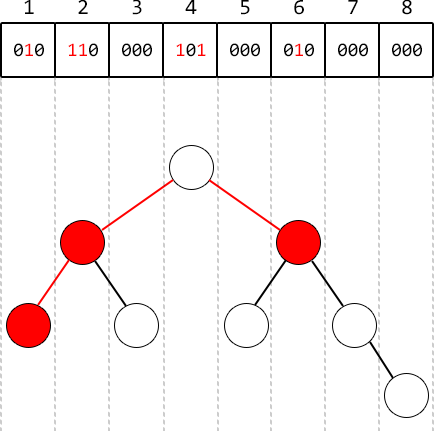
\includegraphics[scale=0.5]{csc263-a1-q3-illustration}
                \caption{Illustrated array for the provided data structure, storing the set $\{1, 2, 6\}$ with $n = 8$.}
                \end{center}
            \end{figure}

        In implementations, bitwise tests (denoted as logical intersections and unions here) can be done on nodes to test various conditions. This data structure requests $3n$ bits of storage, which is clearly in $O(n)$. The tree transversal logic is slightly more complicated than a standard binary-tree-in-array where the head is stored at index $1$, however it's quite doable.

        \item [(b)] To retrieve the maximum value, we can used a recursive function defined like so:
            \begin{enumerate}
            \item [(a)] Set $\texttt{node} = \lfloor n / 2 \rfloor$.
            \item [(b)] $\texttt{A[node]} = 000$, throw an error, the set is empty.
            \item [(c)] If the node has a right subtree ($\texttt{A[node]} \cap 001 == 001$), set $\texttt{node} = \texttt{subtree}$ and go to \textbf{(c)}.
            \item [(d)] Otherwise if the node exists ($\texttt{A[node]} \cap 010 == 010$), return \texttt{node} (which corresponds to the value of the set item).
            \item [(e)] Otherwise if the node has a left subtree ($\texttt{A[node]} \cap 100 == 100$), set $\texttt{node} = \texttt{subtree}$ and go to \textbf{(c)}.
            \end{enumerate}
            This operation recurses from the root down the tree and can go as far as the furthest node--that is, the height of the tree. The height of a balanced binary trees is in $O(\log n)$, so therefore the number of steps the algorithm takes is also in $O(\log n)$. \\

            For $\texttt{node} \in \{1, 2, ..., n\}$ insertion algorithm can be defined as follows:
            \begin{enumerate}
            \item [(a)] Activate the item at index \texttt{node}: $\texttt{A[node]} = \texttt{A[node]} \cup 010$
            \item [(b)] Set $\texttt{parent} = \texttt{node}$.
            \item [(c)] If the \texttt{parent} is the root element ($\texttt{node} = \lfloor n / 2 \rfloor$), return.
            \item [(d)] Otherwise, set \texttt{parent} to its respective parent node.
            \item [(c)] If we came from the left subtree, activate \texttt{parent}'s left bit: $\texttt{A[parent]} = \texttt{A[parent]} \cup 100$.
            \item [(d)] Otherwise if we came from the right subtree, activate \texttt{parent}'s right bit: $\texttt{A[parent]} = \texttt{A[parent]} \cup 001$.
            \item [(e)] Go to \textbf{(c)}.
            \end{enumerate}

            The worse-case run time of insertion is when we insert a leaf of the tree. In this case, we recurse up to the root of the tree a number of steps corresponding to the tree's height. Therefore this too is in $O(\log n)$.

        \item [(c)] Insertion is a trivial bitwise comparison. Given $\texttt{node} \in \{1, 2, ..., n\}$, we return true if $\texttt{A[node]} \cap 010 == 010$, false otherwise. Looking up an item in an array by its index is a constant time operation, and the comparison also requires a constant time. Therefore, the membership test is in $O(1)$.
    \end{enumerate}
\end{enumerate}
\end{document}
